% chap4.tex
%

\mychapter{Non-factoid Question Answering}

Most of the questions that people have are not factoid and cannot be simply answered with a name, date or a number.
Typically, such questions require a more elaborate fragment of text as an answer.
Traditionally, question answering systems turn to web documents that might contain some relevant passages to be used as an answer.

\noindent
In this chapter, I summarize the proposed work for improving automatic non-factoid question answering by better understanding the structure of web documents and relationships between their parts and fragments.
% In particular, we first focus on ...., and then try to ...
% The goal is 

\section{Utilizing the Structure of Web Pages}

Non-factoid questions are typically answered with a relatively long paragraph of text\footnote{TREC LiveQA'15 challenge limits the answer to 1000 characters}.
This fact and the nature of questions limits the utility of structured KB resources.
One of the main challenges for non-factoid question answering is matching between the question needs and the information expressed in text fragment.
Analysis of TREC LiveQA 2015 participants \cite{savenkov_liveqa15} revealed that the quality of answers extracted from previously posted similar questions is typically higher than from regular web passages.
Therefore, non-factoid QA system would benefit from the information on which questions does a paragraph of text answer.
This information can often be extracted from the structure of a web document, e.g. forum threads, FAQ pages or various CQA websites.
Alternatively, we can train a model to predict whether a paragraph answers a given question using titles, subtitles and surrounding text of a web page.

\begin{figure}[h]
\centering
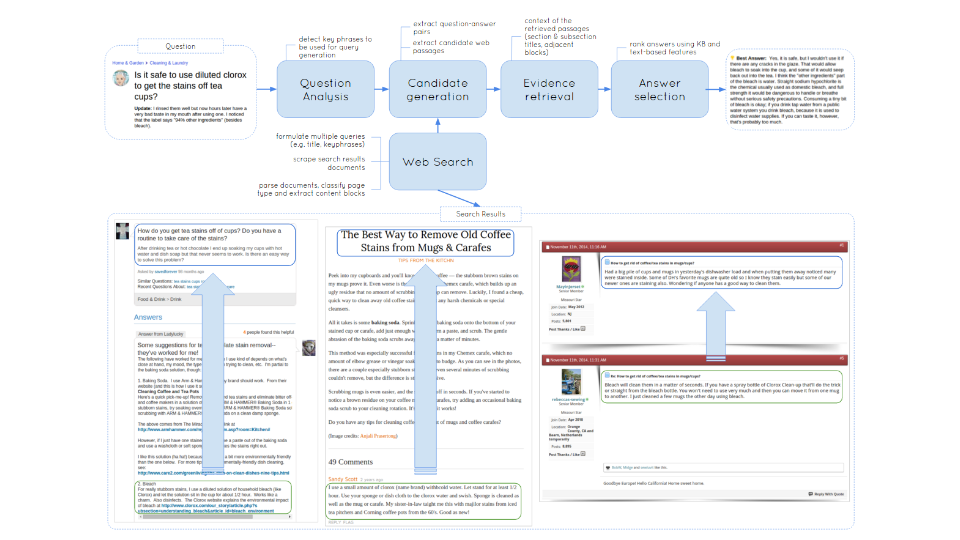
\includegraphics[width=\textwidth]{img/web_page_structure_nonfactoid}
\label{fig:web_page_structure_nonfactoid}
\caption{Using web page structure information for non-factoid question answering}
\end{figure}

My proposal for non-factoid question answering can be summarized as follows:
\begin{itemize}
\setlength\itemsep{0em}
\item \textbf{CQA candidate generation}: retrieve a set of question-answer pairs by searching a CQA archive\footnote{https://answers.yahoo.com/}
\item \textbf{Web document retrieval}: retrieve a set of documents by querying web search with the question (and queries generated from it)
\item \textbf{Web candidate answer generation}: classify web page into one of the following types: article, forum thread, FAQ page, CQA page, other. Extract key elements using type-specific extractors (QnA pairs, FAQ and CQA pages, forum question and posts and article passages with the corresponding titles, subtitles and surrounding text).
\item \textbf{Ranking}: Rank the generated candidate answers by building on techniques from existing research \cite{surdeanu2011learning}.
\end{itemize}


\section{Evaluation}
LiveQA


\section{Summary}
